\documentclass{beamer}
\usetheme[hideothersubsections]{PaloAlto}
\usecolortheme{albatross}

\usepackage{etoolbox}

\definecolor{Antra}{RGB}{105,105,105}
\definecolor{AntraB}{RGB}{105,105,125}
\definecolor{Gris}{RGB}{80,80,85}

\setbeamercolor*{structure}{fg=Antra!50,bg=AntraB}
\setbeamercolor*{palette primary}{use=structure,fg=white,bg=Gris}
\setbeamercolor*{background canvas}{bg=Antra,fg=Antra}
\setbeamercolor*{normal text}{bg=AntraB,fg=Antra!10}
\setbeamercolor*{navigation symbols}{bg=AntraB,fg=Antra!10}

\beamertemplatenavigationsymbolsempty


\title[Revue de projet Final]{Projet Aéroglisseur \\Revue de Projet Finale}
\author[]{Florian POUTHIER - Tristan DRUSSEL}
\date{Mai 2020}
\institute{4ème année Génie Électrique \\ INSA Strasbourg}

\setbeamertemplate{footline}
{
	\leavevmode% 
	\begin{beamercolorbox}[wd=0.3333\paperwidth,left,ht=0.025\paperheight,dp=0.0125\paperheight]{palette primary}
	   	\hspace*{2em}\insertauthor
	\end{beamercolorbox}
	\begin{beamercolorbox}[wd=0.3333\paperwidth,center,ht=0.025\paperheight,dp=0.0125\paperheight]{AntraB}
		\hspace*{2em}  \insertframenumber\hspace*{2em}
	\end{beamercolorbox}
	\begin{beamercolorbox}[wd=0.3333\paperwidth,right,ht=0.025\paperheight,dp=0.0125\paperheight]{palette primary}
		\insertshorttitle\hspace*{2em}
	\end{beamercolorbox}
	\vskip0pt
}


\begin{document}
	\begin{frame}[noframenumbering,plain]
		\titlepage
	\end{frame}
	\author[]{Tristan DRUSSEL}
	\begin{frame}
		\frametitle{Aperçu}
	%Contexte du projet
	%organisation du travail,problématique, questionnement reformulation du rpbleme
		\begin{columns}[T]
	  		\begin{column}{0.5\textwidth}
	  		\begin{itemize}
	  			\item Réalisation d'un aéroglisseur sur la base du Chticat
				\item Mise en oeuvre de l'électronique de puissance, de l'électronique numérique et de la mécanique
	  		\end{itemize}
	    	
	  		\end{column}
	  		\begin{column}{0.5\textwidth}
	  			\begin{figure}
	    			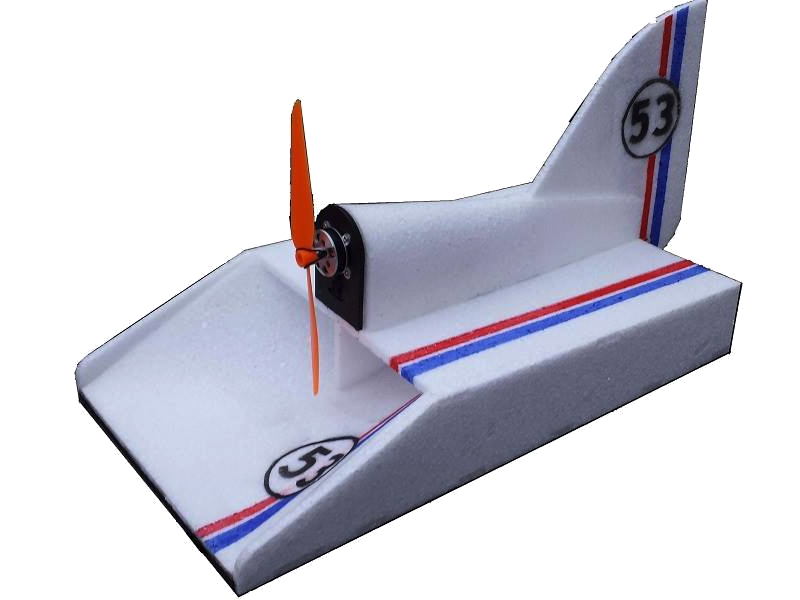
\includegraphics[width=0.8\textwidth]{../Illus/Chticat.png}
	    			\caption{Photo d'un Chticat originel}
	    		 \end{figure}
	  		\end{column}
		\end{columns}
	\end{frame}
	\begin{frame}{Sommaire}
	%Plan d'intervention succinct
		\setcounter{tocdepth}{1}
		\tableofcontents
	\end{frame}
	\begin{frame}{L'aspect mécanique}
		\section[Mécanique]{L'aspect Mécanique}
		\subsection{Modèle CAO}
		\begin{columns}[T]
	  		\begin{column}{0.5\textwidth}
		    	\begin{itemize}
		    		\item Récupération des sources
		    		\item Adaptation du modèle
		    	\end{itemize}
	  		\end{column}
	  		\begin{column}{0.5\textwidth}
	    		\begin{figure}
	    			%\includegraphics[width=0.8\textwidth]{../Illus/3Dview.png}
	    			\caption{Modèle 3D modifié et adapté}
	    		 \end{figure}
	  		\end{column}
		\end{columns}
		
	\end{frame}
	\begin{frame}{Électronique Numérique}
		\section[ENUM]{L'aspect Électronique Numérique}
		Communication entre différents éléments:
		\begin{itemize}
			\item Application mobile
	  		\item Module Bluetooth: \texttt{HC-05}
			\item \texttt{PIC16F1619}
			\item \texttt{dsPIC10F2030}
	  	\end{itemize}
	  	Contrôle de l'onduleur
	\end{frame}
	\begin{frame}{Électronique Numérique:\\Communication Bluetooth}
		\subsection[Bluetooth]{Communication Bluetooth}
		\begin{columns}[T]
	  		\begin{column}{0.5\textwidth}
		    	\begin{itemize}
		    		\item Contrôle à partir du Smartphone
		    	\end{itemize}
		    	\begin{figure}
		    		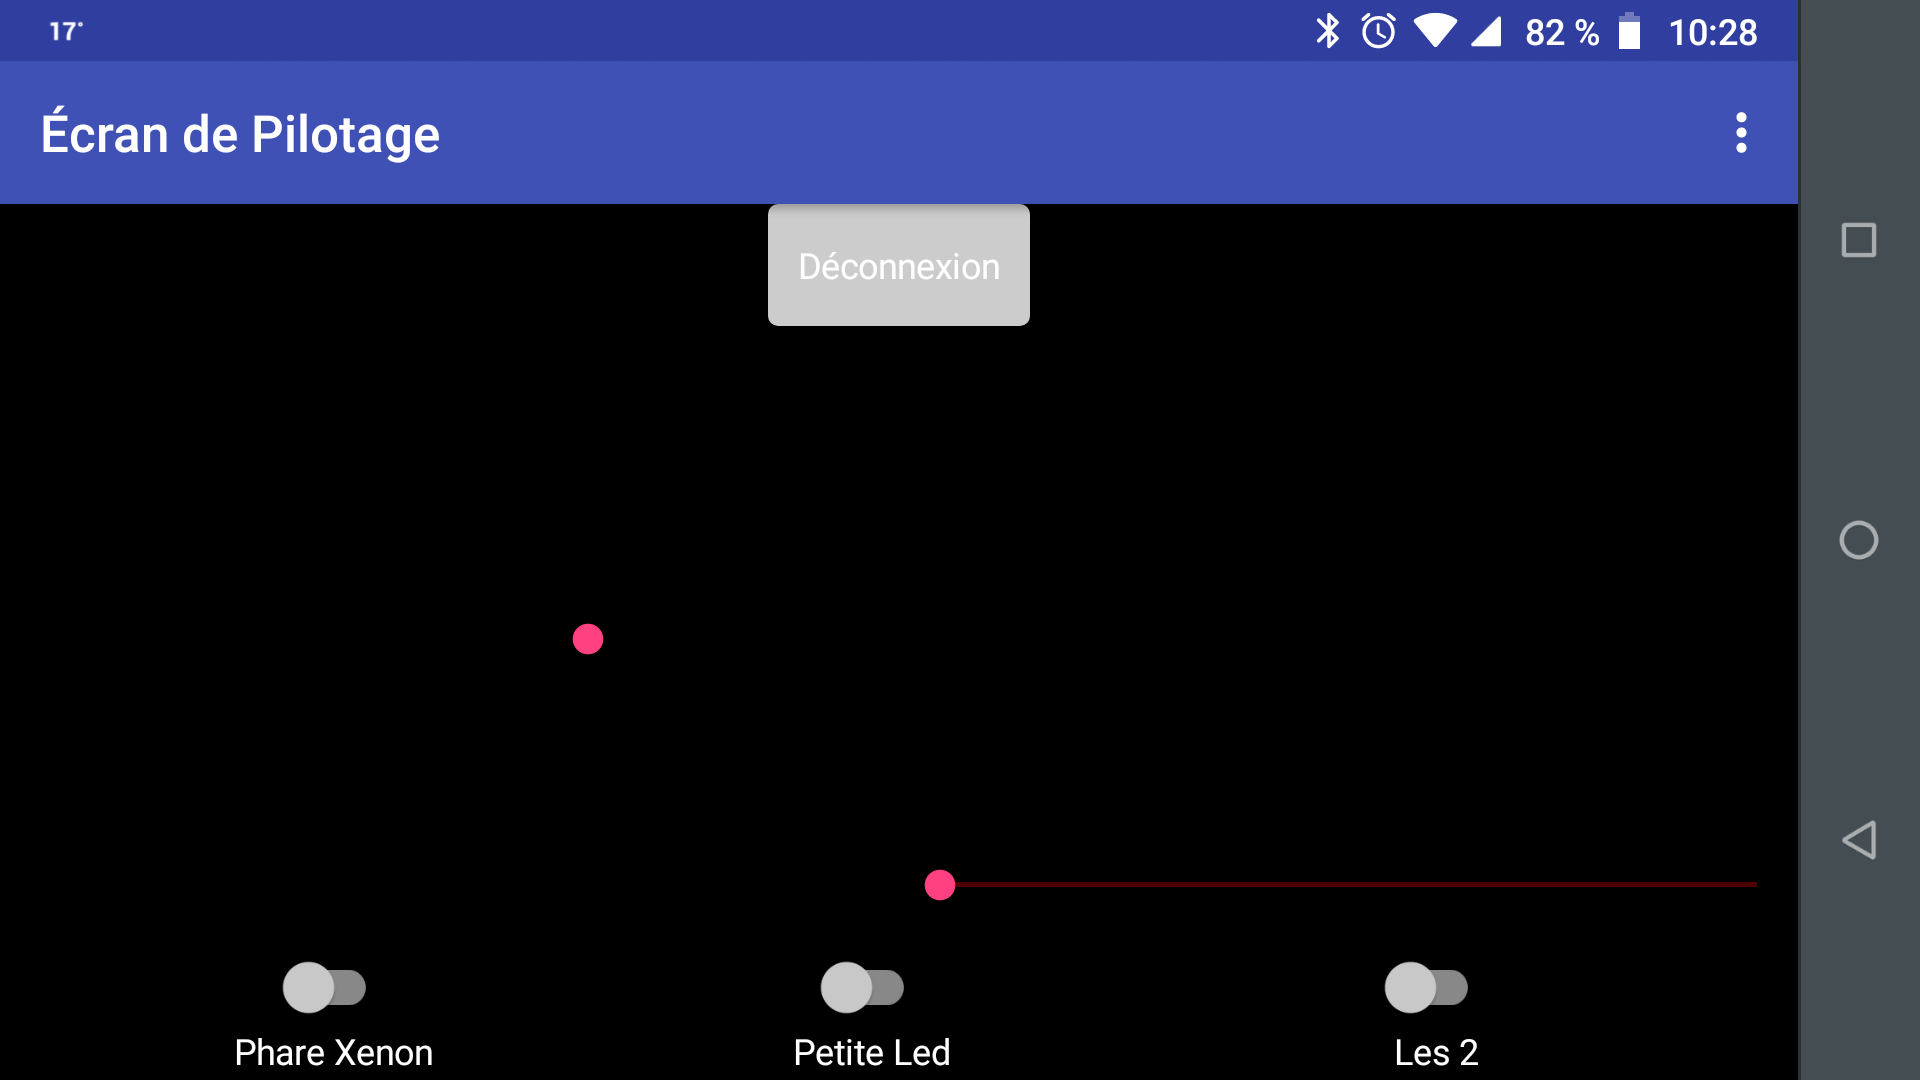
\includegraphics[width=0.8\textwidth]{../Illus/AppPilotage.png}
	    			\caption{Ecran de pilotage de l'application}
	    		 \end{figure}
	  		\end{column}
	  		\begin{column}{0.5\textwidth}
	  			\begin{figure}
	    			\hspace*{2em}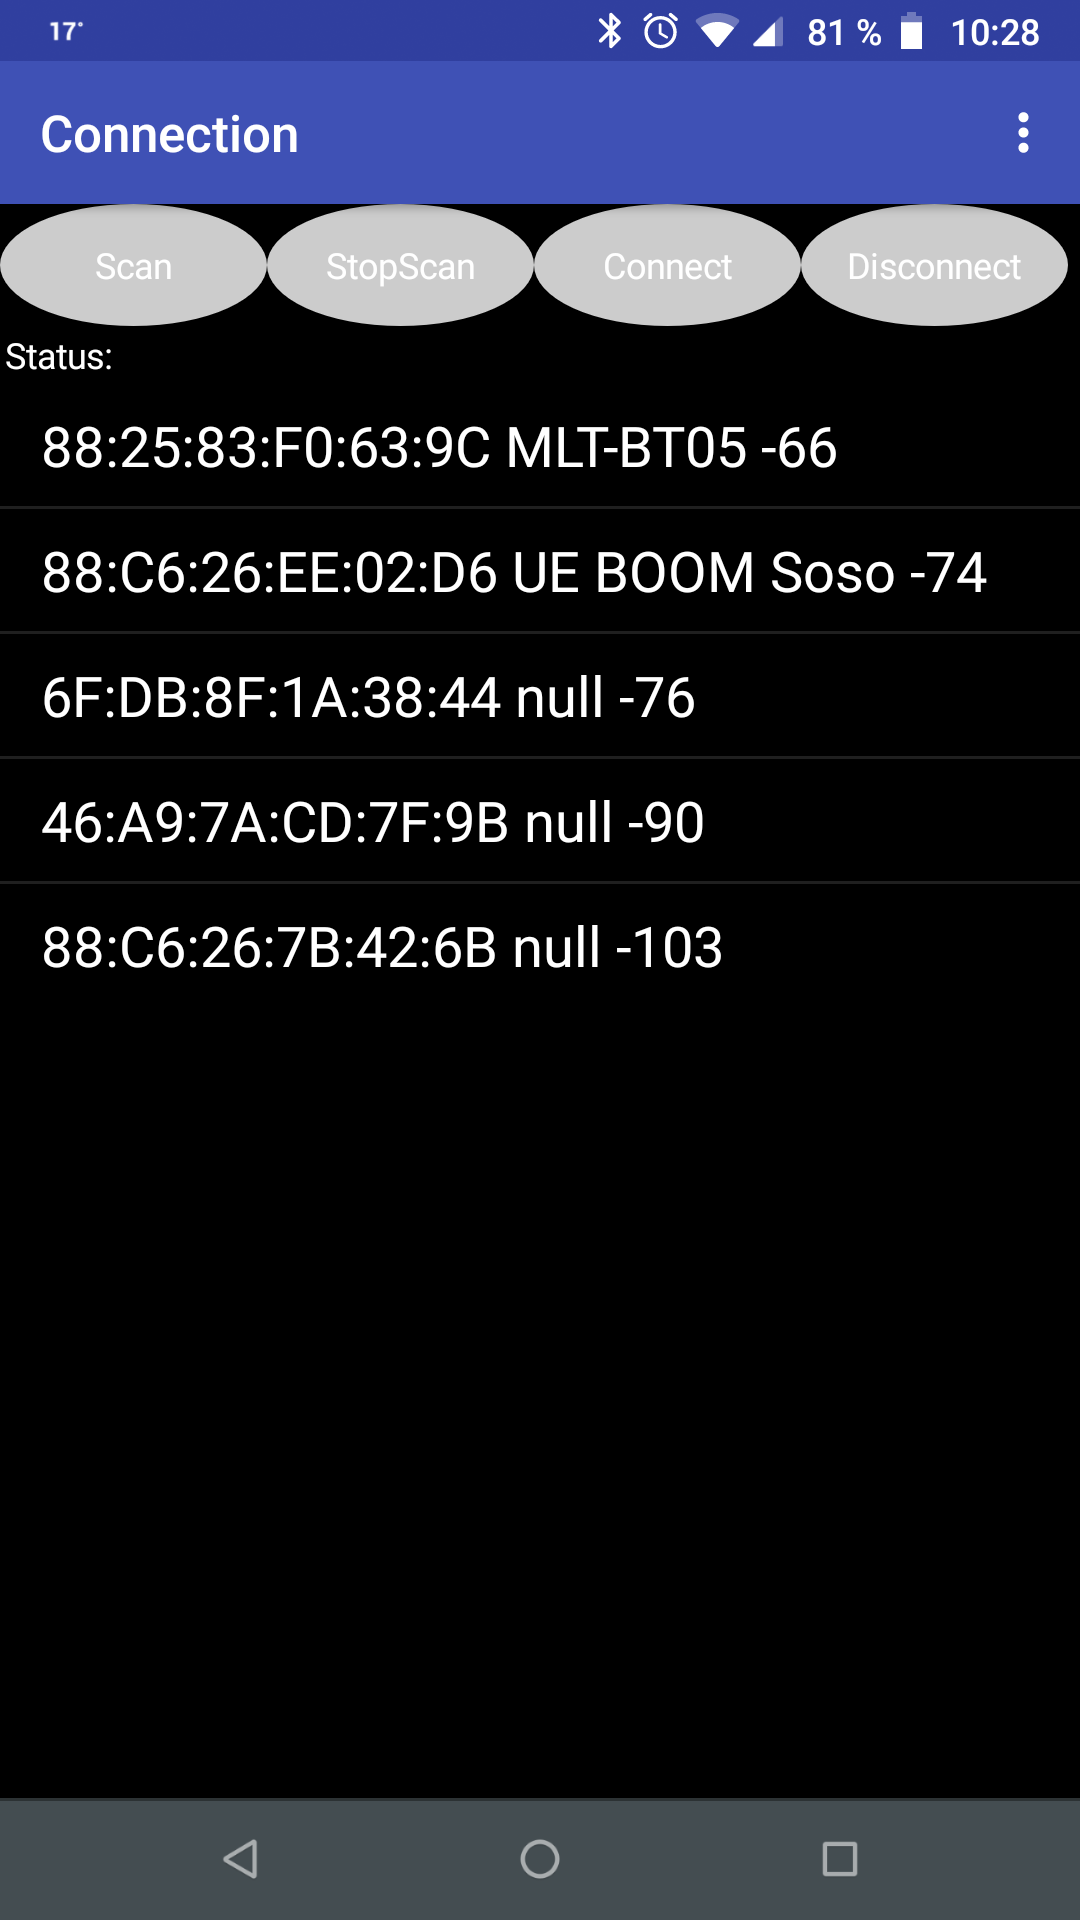
\includegraphics[height=0.8\textheight]{../Illus/AppConnection.png}
	    			\caption{Ecran de connection de l'application}
	    		\end{figure}
	  		\end{column}
		\end{columns}
		
	\end{frame}
	\begin{frame}{Électronique Numérique:\\Communication Série}
		\subsection[Série]{Communication Série}
		\begin{itemize}
		    \item Communication entre le Récepteur Bluetooth et le \texttt{PIC16F1619}
		\end{itemize}
	\end{frame}
	\begin{frame}{Électronique Numérique:\\Communication \textit{Serial Peripheral Interface}}
		\subsection[SPI]{Communication SPI}
		\begin{itemize}
		    \item Communication entre le \texttt{PIC16F1619} et le \texttt{dsPIC10F2030}
		\end{itemize}
	\end{frame}
	
	\author[]{Florian POUTHIER}
	%Intro ENPU
	\begin{frame}{Électronique de Puissance}
		\section[ENPU]{L'aspect Électronique de Puissance}
		Gestion de l'alimentation et mise en oeuvre d'un onduleur triphasé
 		\begin{itemize}
			\item Analyse fonctionnelle
			\item Simulations sous \textit{PSIM}
			\item Conception des PCBs
		\end{itemize}
	\end{frame}
	
	% Modélisation théorique
	\begin{frame}{Électronique de Puissance\\ Analyse fonctionnelle}
		\subsection[Analyse F]{Analyse fonctionnelle}
		\begin{columns}[T]
	  		\begin{column}{0.4\textwidth}
				\begin{itemize}
					\item Structure d'un moteur \textit{brushless}
					\item Lois magnétiques régissant la mise en mouvement du moteur
					\item Circuit électronique permettant le contrôle du moteur
				\end{itemize}
	  		\end{column}
	  		\begin{column}{0.6\textwidth}
	  			\vspace{-1em}
	  			\begin{figure}
	  				\begin{center}
	  					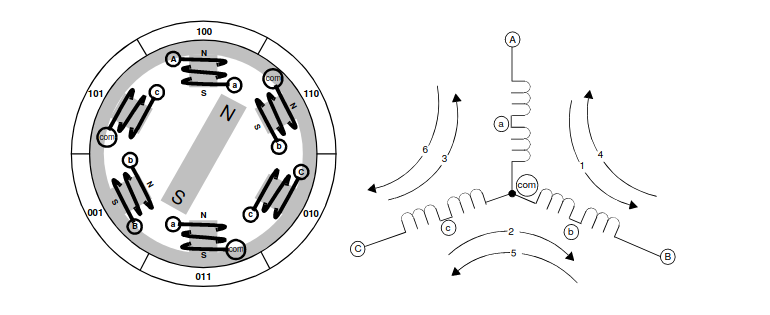
\includegraphics[height=0.3\textheight]{../Illus/struct_bldcm.png}
	  				\end{center}
	    			\caption{Structure et modélisation d'un \textit{moteur brushless}}
	    		\end{figure}
	    		\vspace{-2em}
	  			\begin{figure}
	  				\begin{center}
	  					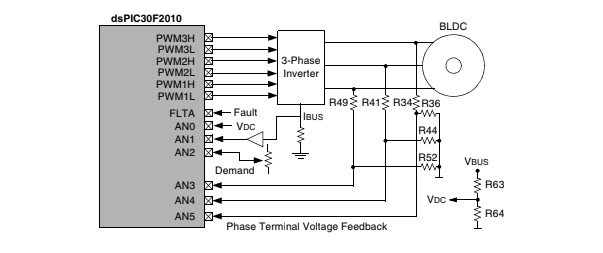
\includegraphics[height=0.3\textheight]{../Illus/back_emf_scheme.png}
	  				\end{center}
	    			\caption{Onduleur et détection de la force contre-électromotrice}
	    		\end{figure}
	  		\end{column}
		\end{columns}

	\end{frame}	
		
	% Simulations PSIM - Alimentation
	\begin{frame}{Électronique de Puissance\\ Simulations sous PSIM}
		\subsection[Simulations]{Simulations sous PSIM}
		Simulation de fonctionnement de l'alimentation
		\begin{itemize}
			\item Mise en oeuvre du schéma de principe interne du composant d'alimentation de type convertisseur \textit{Buck}
			\item Dimensionnement adéquat des composants externes au convertisseur
			\item Validation du modèle et des valeurs retenues pour les composants externes
		\end{itemize}
	\end{frame}	
	
	% Simulations PSIM - BLDCM
	\begin{frame}
		Simulation de fonctionnement du moteur \textit{brushless}
		\begin{itemize}
			\item Étude du pilotage d'un moteur \textit{brushless}
			\item Prise en compte des aspects mécaniques avec une modélisation mathématique de l'hélice
			\item Vérification du fonctionnement et des performances de propulsion espérées
		\end{itemize}
	\end{frame}	
	
	% Conception des PCBs - Carte Alim
	\begin{frame}{Électronique de Puissance\\ Conception des cartes électroniques}
		\subsection[PCBs]{Conception des cartes électroniques}
		\begin{columns}[T]
	  		\begin{column}{0.5\textwidth}
	  			Interface d'alimentation
		    	\begin{itemize}
		    		\item Obtention de toutes les tensions nécessaires au fonctionnement du système
		    		\item Masse routée pour éviter des retours de courant destructeurs
		    		\item Optimisation du placement des composants afin d'éviter des conflits EM
		    	\end{itemize}
	  		\end{column}
	  		\begin{column}{0.5\textwidth}
	  			\begin{figure}
	  				\begin{center}
	  					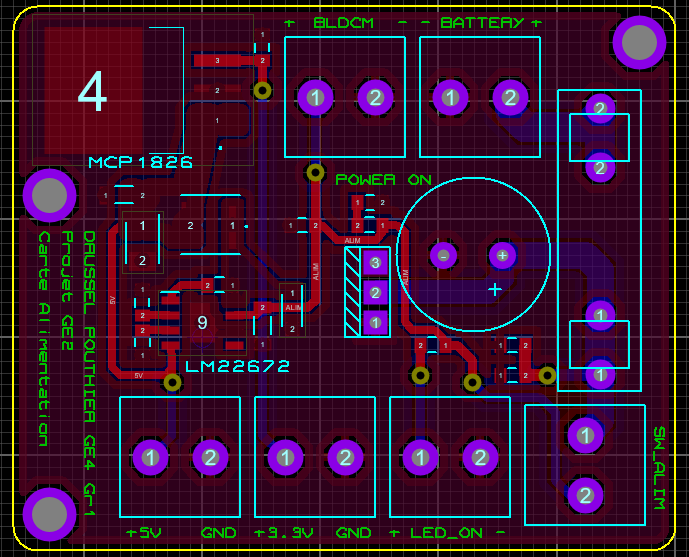
\includegraphics[height=0.5\textheight]{../Illus/PCB_Alim.PNG}
	  				\end{center}
	    			\caption{Vue de la carte interface d'alimentation}
	    		\end{figure}
	  		\end{column}
		\end{columns}
	\end{frame}

	% Conception des PCBs - Carte Bras de pont
	\begin{frame}{Électronique de Puissance\\ Conception des cartes électroniques}
		\begin{columns}[T]
	  		\begin{column}{0.6\textwidth}
	  			Bras de pont triphasés
		    	\begin{itemize}
		    		\item Détermination des surfaces d'échanges thermiques adéquates aux pertes des MOSFETs
		    		\item Driver de MOSFETs pour la liaison entre les signaux de PWM et la commutation des transistors
		    		\item Condensateur de découplage afin d'éviter des retours de courant vers l'alimentation
		    	\end{itemize}
	  		\end{column}
	  		\begin{column}{0.4\textwidth}
	  			\begin{figure}
	  				\begin{center}
	  					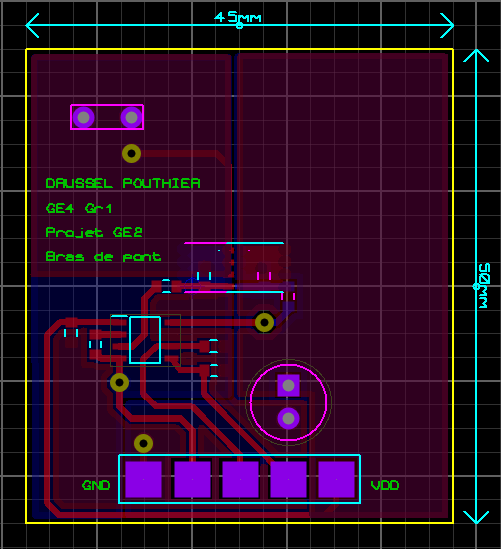
\includegraphics[height=0.5\textheight]{../Illus/PCB_Bras_de_pont.PNG}
	  				\end{center}
	    			\caption{Vue de la carte bras de pont}
	    		\end{figure}
	  		\end{column}
		\end{columns}
	\end{frame}
	
	% Conception des PCBs - Carte commande
	\begin{frame}{Électronique de Puissance\\ Conception des cartes électroniques}
		\begin{columns}[T]
	  		\begin{column}{0.5\textwidth}
	  			Commande générale
		    	\begin{itemize}
		    		\item Mise en oeuvre de deux microcontrolleurs PIC
		    		\item Un microcontroleur pour la gestion des informations utilisateur
		    		\item Un microcontroleur pour le contrôle de l'onduleur
		    		\item Réception d'ordres via Bluetooth et commande de l'onduleur et du servomoteur en fonction
		    	\end{itemize}
	  		\end{column}
	  		\begin{column}{0.5\textwidth}
	  			\begin{figure}
	  				\begin{center}
	  					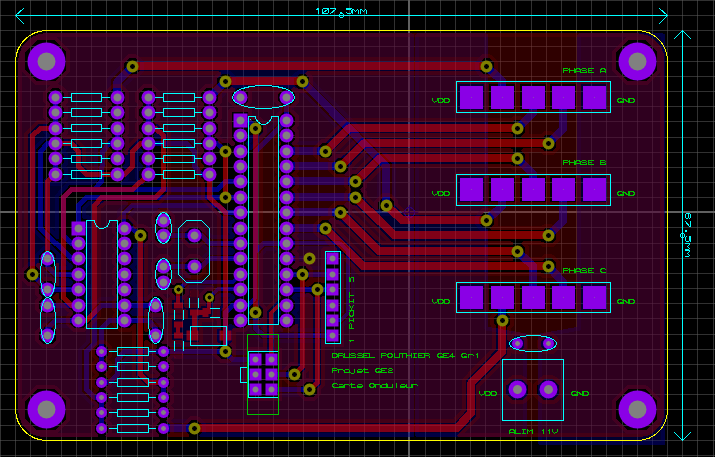
\includegraphics[height=0.4\textheight]{../Illus/PCB_Onduleur.PNG}
	  				\end{center}
	    			\caption{Vue de la carte de commande générale}
	    		\end{figure}
	  		\end{column}
		\end{columns}
	\end{frame}
	
	\begin{frame}{Pursuites du projet}
		\section[Poursuites]{Poursuites du projet}
		\begin{itemize}
		    \item Pilotage de l'onduleur
		    \item Réalisation des cartes	
		    \item Tests en conditions réelles
		\end{itemize}
	\end{frame}
	
	\begin{frame}{Conclusion}
	\section*{Conclusion}
	%Conclusion
	\begin{itemize}
		    \item Projet multidisciplinaire
		    \item Mise en oeuvre des compétences acquises précédements
		\end{itemize}
	\end{frame}
	\author[]{Florian POUTHIER - Tristan DRUSSEL}
	\begin{frame}[plain]{Merci de votre attention}
	\section*{}
		%remerciement
		\titlepage
	\end{frame}
\end{document}